\chapter{Real-World System Examples}
\label{ch:real-world-systems}

\begin{nontechnical}
\textbf{Real systems are like complete orchestras}---not just one instrument, but all concepts working together in harmony.

\textbf{Simple idea:}
\begin{itemize}
\item WiFi = OFDM + MIMO + smart antenna switching (fast, short range)
\item LTE = cellular towers + adaptive modulation (medium speed, wide area)
\item GPS = weak satellite signals + spread spectrum (navigation, global)
\item Bluetooth = frequency hopping + low power (personal devices)
\item LoRa = chirp signals + ultra-long range (IoT sensors, years on battery)
\end{itemize}

\textbf{Real use:} These are the systems in your phone, car, home. Each optimizes different trade-offs: speed vs range vs power.

\textbf{Why study complete systems?} Theory is one thing, but real implementations face constraints: regulations, cost, battery life, interference. Understanding complete systems shows how theory becomes practice.
\end{nontechnical}

\section{Overview}

This chapter provides \textbf{end-to-end analysis} of deployed communication systems, demonstrating how fundamental concepts---modulation, coding, synchronization, equalization, and link budgets---integrate into practical implementations.

\begin{keyconcept}
Real-world systems make fundamental \textbf{trade-offs between competing requirements}: data rate, range, power consumption, latency, and cost. No single system optimizes all parameters; each is engineered for specific use cases and regulatory constraints.
\end{keyconcept}

\textbf{Systems analyzed in this chapter:}
\begin{enumerate}
\item \textbf{WiFi 802.11n} (Wireless LAN)---high throughput, indoor coverage
\item \textbf{LTE} (4G Cellular)---wide-area mobility with adaptive coding
\item \textbf{DVB-S2X} (Satellite TV)---long-distance broadcast from GEO
\item \textbf{GPS L1 C/A} (Navigation)---sub-noise signal acquisition
\item \textbf{Bluetooth 5.0} (Personal Area Network)---low power, frequency hopping
\item \textbf{LoRaWAN} (IoT)---ultra-long range with minimal power
\end{enumerate}

Each analysis includes: physical layer parameters, modulation and coding schemes, link budget calculations, synchronization methods, equalization techniques, and measured performance.

\section{WiFi 802.11n: High-Throughput WLAN}
\label{sec:wifi}

\subsection{System Parameters}

\begin{tabular}{@{}ll@{}}
\toprule
\textbf{Parameter} & \textbf{Value} \\
\midrule
Standard & IEEE 802.11n (2009) \\
Frequency bands & 2.4~GHz, 5~GHz \\
Channel bandwidth & 20~MHz, 40~MHz \\
MIMO configuration & $2 \times 2$, $3 \times 3$, $4 \times 4$ \\
Modulation & BPSK to 64-QAM (per subcarrier) \\
Multiple access & OFDMA + CSMA/CA \\
FEC coding & Convolutional ($K = 7$, rates: $\frac{1}{2}, \frac{2}{3}, \frac{3}{4}, \frac{5}{6}$) \\
Peak data rate & 150~Mbps (1 stream), 600~Mbps (4 streams) \\
\bottomrule
\end{tabular}

\subsection{OFDM Physical Layer}

WiFi 802.11n employs \textbf{Orthogonal Frequency Division Multiplexing (OFDM)} to combat multipath fading in indoor environments.

\textbf{OFDM parameters (20~MHz channel):}
\begin{itemize}
\item FFT size: $N_{\text{FFT}} = 64$
\item Total subcarriers: 64 (52 data + 4 pilots + 8 guard/DC)
\item Subcarrier spacing: $\Delta f = 312.5$~kHz
\item Symbol duration: $T_{\text{sym}} = 3.2~\mu$s (data) + $0.8~\mu$s (guard interval) = $4~\mu$s
\item Guard interval: $T_g = 0.8~\mu$s ($\frac{1}{4}$ symbol, handles up to 240~m delay spread)
\end{itemize}

The OFDM symbol duration is calculated as:
\begin{equation}
T_{\text{sym}} = \frac{1}{\Delta f} = \frac{1}{312.5 \times 10^3} = 3.2~\mu\text{s}
\end{equation}

\textbf{40~MHz channel} doubles capacity:
\begin{itemize}
\item FFT size: $N_{\text{FFT}} = 128$
\item Data subcarriers: 108 (2.08$\times$ increase)
\end{itemize}

\begin{center}
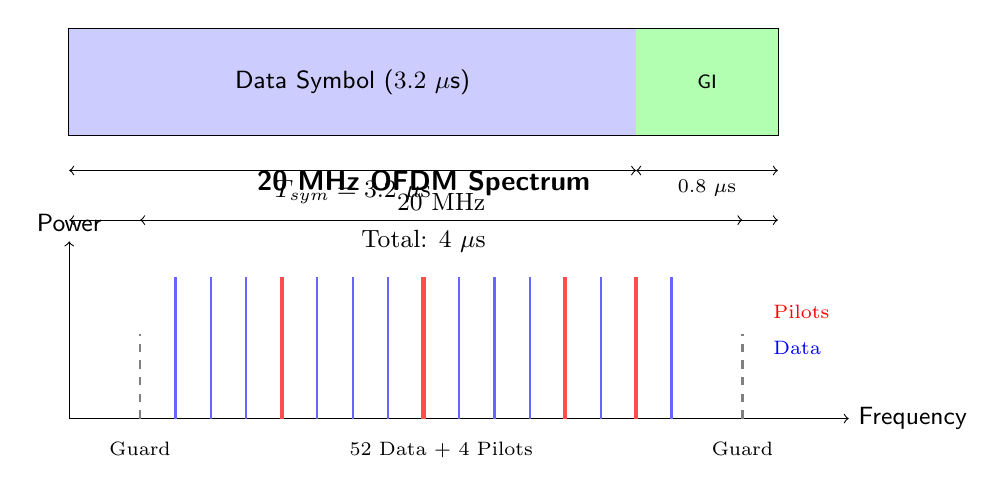
\begin{tikzpicture}[scale=0.9]
% OFDM Symbol Structure
\draw[thick] (0,0) rectangle (10,1.5);
\fill[blue!20] (0,0) rectangle (8,1.5);
\fill[green!30] (8,0) rectangle (10,1.5);

\node at (4,0.75) {\sffamily\small Data Symbol ($3.2~\mu$s)};
\node at (9,0.75) {\sffamily\scriptsize GI};

% Dimensions
\draw[<->] (0,-0.5) -- (8,-0.5) node[midway,below] {\small $T_{\text{sym}} = 3.2~\mu$s};
\draw[<->] (8,-0.5) -- (10,-0.5) node[midway,below] {\scriptsize $0.8~\mu$s};
\draw[<->] (0,-1.2) -- (10,-1.2) node[midway,below] {\small Total: $4~\mu$s};

% Frequency domain representation
\begin{scope}[shift={(0,-4)}]
\node[above] at (5,3) {\sffamily\bfseries 20~MHz OFDM Spectrum};
\draw[->] (0,0) -- (11,0) node[right] {\sffamily\small Frequency};
\draw[->] (0,0) -- (0,2.5) node[above] {\sffamily\small Power};

% Subcarriers
\foreach \x in {1.5,2,2.5,3,3.5,4,4.5,5,5.5,6,6.5,7,7.5,8,8.5} {
  \draw[thick,blue!60] (\x,0) -- (\x,2);
}
% Pilot subcarriers (highlighted)
\draw[thick,red!70,line width=1.5pt] (3,0) -- (3,2);
\draw[thick,red!70,line width=1.5pt] (5,0) -- (5,2);
\draw[thick,red!70,line width=1.5pt] (7,0) -- (7,2);
\draw[thick,red!70,line width=1.5pt] (8,0) -- (8,2);

% Guard bands
\draw[thick,gray,dashed] (1,0) -- (1,1.2);
\draw[thick,gray,dashed] (9.5,0) -- (9.5,1.2);

% Labels
\node[below,font=\scriptsize] at (1,-0.2) {Guard};
\node[below,font=\scriptsize] at (5.25,-0.2) {52 Data + 4 Pilots};
\node[below,font=\scriptsize] at (9.5,-0.2) {Guard};
\node[right,font=\scriptsize,red] at (9.8,1.5) {Pilots};
\node[right,font=\scriptsize,blue] at (9.8,1) {Data};

\draw[<->] (1,2.8) -- (9.5,2.8) node[midway,above,font=\small] {20~MHz};
\end{scope}
\end{tikzpicture}
\end{center}

\begin{calloutbox}[colback=blue!5!white,colframe=blue!75!black]{Why OFDM for WiFi?}
Indoor wireless channels exhibit severe \textbf{multipath propagation}---signals reflect off walls, furniture, and people, creating multiple delayed copies. In a traditional single-carrier system, these reflections cause intersymbol interference (ISI).

OFDM solves this by:
\begin{itemize}
\item Dividing the channel into narrow subcarriers (312.5~kHz each)
\item Each subcarrier experiences flat fading (no ISI within narrow band)
\item Guard interval absorbs multipath delays up to $0.8~\mu$s (240~m)
\item Simple per-subcarrier equalization (single complex division)
\end{itemize}

Trade-off: Guard interval reduces efficiency by 20\%, but eliminates complex time-domain equalization.
\end{calloutbox}

\subsubsection{Frame Structure}\label{frame-structure}

\begin{verbatim}
[Preamble] [SIGNAL] [Data Field]
    |         |          |
  20 s     4 s    Variable
\end{verbatim}

\textbf{Legacy preamble} (20 \$\textbackslash mu\$s): - Short training
(8 \$\textbackslash mu\$s): AGC, coarse CFO - Long training (8
\$\textbackslash mu\$s): Fine CFO, channel estimation - SIGNAL field (4
\$\textbackslash mu\$s): Rate, length (BPSK, rate 1/2)

\textbf{HT preamble} (for 802.11n): - HT-SIG (8 \$\textbackslash mu\$s):
MCS, bandwidth, MIMO streams - HT-LTF (4 \$\textbackslash mu\$s
\$\textbackslash times\$ Nss): Channel estimation per spatial stream

\begin{center}\rule{0.5\linewidth}{0.5pt}\end{center}

\subsubsection{Modulation \& Coding Schemes
(MCS)}\label{modulation-coding-schemes-mcs}

\textbf{20 MHz, 1 spatial stream}:

{\def\LTcaptype{} % do not increment counter
\begin{longtable}[]{@{}lllll@{}}
\toprule\noalign{}
MCS & Modulation & Code Rate & Data Rate (Mbps) & Usage \\
\midrule\noalign{}
\endhead
\bottomrule\noalign{}
\endlastfoot
0 & BPSK & 1/2 & 6.5 & Max range, poor SNR \\
1 & QPSK & 1/2 & 13 & Long range \\
2 & QPSK & 3/4 & 19.5 & \\
3 & 16-QAM & 1/2 & 26 & Medium range \\
4 & 16-QAM & 3/4 & 39 & \\
5 & 64-QAM & 2/3 & 52 & Short range, good SNR \\
6 & 64-QAM & 3/4 & 58.5 & \\
7 & 64-QAM & 5/6 & 65 & Max throughput \\
\end{longtable}
}

\textbf{40 MHz, 2 spatial streams}: 2\$\textbackslash times\$ data rate
\$\textbackslash rightarrow\$ 150 Mbps (MCS 15)

\textbf{40 MHz, 4 spatial streams}: 4\$\textbackslash times\$ data rate
\$\textbackslash rightarrow\$ 600 Mbps (MCS 31, 64-QAM 5/6)

\begin{center}\rule{0.5\linewidth}{0.5pt}\end{center}

\subsection{Link Budget Analysis: Indoor WiFi}

\textbf{Scenario:} 10~m indoor link at 2.4~GHz, 20~MHz bandwidth

\subsubsection*{Given Parameters}

\begin{tabular}{@{}ll@{}}
TX power & $P_t = 20$~dBm (100~mW) \\
TX antenna gain & $G_t = 2$~dBi (omnidirectional) \\
RX antenna gain & $G_r = 2$~dBi \\
Distance & $d = 10$~m \\
Frequency & $f = 2.4$~GHz \\
Bandwidth & $B = 20$~MHz \\
Noise figure & $NF = 6$~dB \\
Wall penetration loss & $L_{\text{wall}} = 5$~dB (single interior wall) \\
\end{tabular}

\subsubsection*{Step 1: Free-Space Path Loss}

\begin{equation}
\text{FSPL\,[dB]} = 20\log_{10}(d_{\text{m}}) + 20\log_{10}(f_{\text{MHz}}) + 32.45
\end{equation}
\begin{equation}
\text{FSPL} = 20\log_{10}(10) + 20\log_{10}(2400) + 32.45 = 20 + 67.6 + 32.45 = 40.05~\text{dB}
\end{equation}

\subsubsection*{Step 2: Total Path Loss}

Including wall penetration:
\begin{equation}
L_{\text{total}} = \text{FSPL} + L_{\text{wall}} = 40.05 + 5 = 45.05~\text{dB}
\end{equation}

\subsubsection*{Step 3: Received Signal Power}

\begin{equation}
P_r = P_t + G_t + G_r - L_{\text{total}}
\end{equation}
\begin{equation}
P_r = 20 + 2 + 2 - 45.05 = -21.05~\text{dBm}
\end{equation}

\subsubsection*{Step 4: Noise Power}

The noise floor for a 20~MHz bandwidth is:
\begin{equation}
N = -174 + 10\log_{10}(B) + NF
\end{equation}
\begin{equation}
N = -174 + 10\log_{10}(20 \times 10^6) + 6 = -174 + 73.0 + 6 = -95.0~\text{dBm}
\end{equation}

where $-174$~dBm/Hz is the thermal noise floor at 290~K.

\subsubsection*{Step 5: Signal-to-Noise Ratio}

\begin{equation}
\text{SNR} = P_r - N = -21.05 - (-95.0) = 73.95~\text{dB}
\end{equation}

\subsubsection*{Step 6: MCS Selection and Data Rate}

With 74~dB SNR, the link can support the highest MCS:
\begin{itemize}
\item \textbf{MCS 7:} 64-QAM, code rate $\frac{5}{6}$
\item \textbf{Required SNR:} $\sim$25~dB
\item \textbf{Link margin:} $74 - 25 = 49$~dB (excellent!)
\item \textbf{Data rate:} 65~Mbps (20~MHz, 1 spatial stream)
\end{itemize}

\begin{calloutbox}{Link Budget Summary}
\textbf{Result: Link closes with 49~dB margin}

This enormous margin provides:
\begin{itemize}
\item Robustness against fading (Rayleigh/Rician)
\item Additional wall penetration capability
\item Support for maximum data rate (MCS 7)
\item Tolerance for multipath and interference
\end{itemize}

\textbf{Practical outcome:} At 10~m indoor range, WiFi operates in a power-rich regime. Range is typically limited by collision domain (CSMA/CA) and AP density, not SNR.
\end{calloutbox}

\subsubsection{Synchronization}\label{synchronization}

\textbf{CFO tolerance}: \$\textbackslash pm\$20 ppm - @ 2.4 GHz:
\$\textbackslash pm\$48 kHz - Subcarrier spacing: 312.5 kHz - Normalized
CFO: \$\textbackslash pm\$0.15 (15\%)

\textbf{Correction}: 1. \textbf{Coarse CFO}: Short preamble
autocorrelation (\$\textbackslash pm\$156 kHz range) 2. \textbf{Fine
CFO}: Long preamble phase difference (\$\textbackslash pm\$10 kHz
accuracy) 3. \textbf{Tracking}: Pilot subcarriers (every OFDM symbol)

\textbf{Timing}: Long preamble correlation peak

\textbf{Channel estimation}: Long preamble (2 known OFDM symbols)

\subsection{Channel Equalization}

\subsubsection*{Single-Antenna (SISO) Equalization}

Each OFDM subcarrier experiences flat fading and can be equalized independently:
\begin{equation}
\hat{S}_k = \frac{R_k}{H_k}
\end{equation}
where:
\begin{itemize}
\item $R_k$ = received symbol on subcarrier $k$
\item $H_k$ = complex channel coefficient (from pilot estimation)
\item $\hat{S}_k$ = equalized symbol estimate
\end{itemize}

\textbf{Channel estimation:} Long training symbols (LTS) in preamble provide known reference:
\begin{equation}
\hat{H}_k = \frac{R_k^{\text{LTS}}}{S_k^{\text{LTS}}}
\end{equation}

\textbf{Pilot tracking:} Four pilot subcarriers per OFDM symbol enable:
\begin{itemize}
\item Phase tracking (common phase error correction)
\item Frequency offset compensation
\item Linear interpolation for data subcarrier channel estimates
\end{itemize}

\subsubsection*{MIMO Equalization ($2 \times 2$)}

For spatial multiplexing, the received signal model per subcarrier is:
\begin{equation}
\mathbf{R} = \mathbf{H} \mathbf{S} + \mathbf{N}
\end{equation}
where $\mathbf{H}$ is the $2 \times 2$ channel matrix.

The \textbf{MMSE equalizer} balances noise amplification:
\begin{equation}
\hat{\mathbf{S}} = \left(\mathbf{H}^H \mathbf{H} + \sigma^2 \mathbf{I}\right)^{-1} \mathbf{H}^H \mathbf{R}
\end{equation}
where $\sigma^2$ is the noise variance.

\textbf{Computational complexity:}
\begin{itemize}
\item $2 \times 2$ matrix inversion per subcarrier
\item 52 subcarriers (20~MHz) $\rightarrow$ 52 inversions per symbol
\item Symbol rate: 250,000 symbols/second
\item Total: $\sim$13 million matrix operations/second
\end{itemize}

\begin{center}
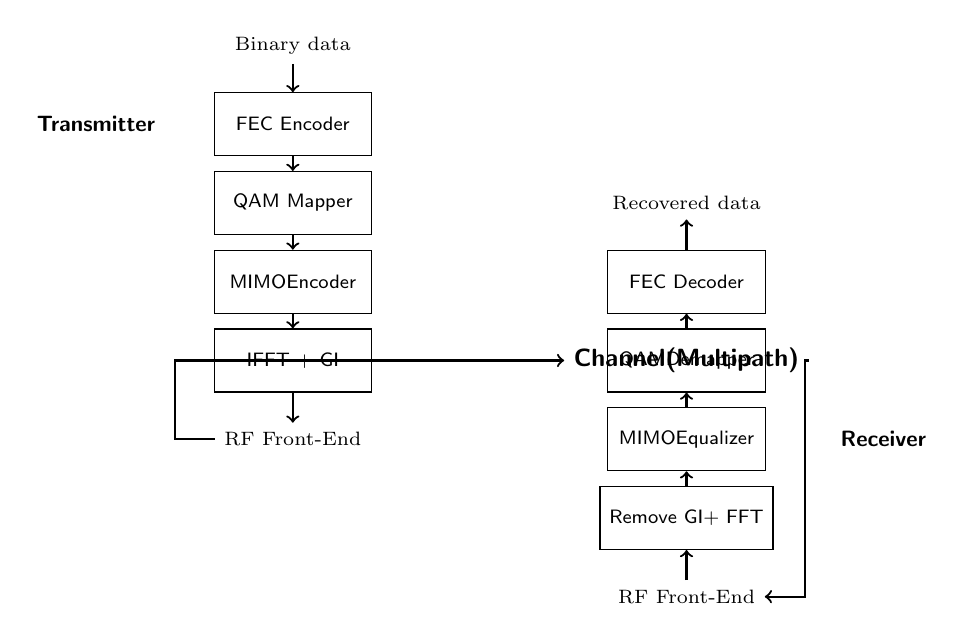
\begin{tikzpicture}[
  block/.style={rectangle, draw, minimum width=2cm, minimum height=0.8cm, font=\sffamily\scriptsize},
  node distance=1.5cm,
  font=\small
]
% Transmit chain
\node (bits) {\scriptsize Binary data};
\node[block, below of=bits, node distance=1cm] (fec) {FEC Encoder};
\node[block, below of=fec, node distance=1cm] (qam) {QAM Mapper};
\node[block, below of=qam, node distance=1cm] (mimo) {MIMO\\Encoder};
\node[block, below of=mimo, node distance=1cm] (ifft) {IFFT + GI};
\node[below of=ifft, node distance=1cm] (rf) {\scriptsize RF Front-End};

% Channel
\node[right of=ifft, node distance=5cm] (channel) {\sffamily\bfseries Channel\\(Multipath)};
\draw[->,thick] (rf) -- ++(-1.5,0) |- (channel);

% Receive chain
\node[below of=channel, node distance=3cm] (rf2) {\scriptsize RF Front-End};
\node[block, above of=rf2, node distance=1cm] (fft) {Remove GI\\+ FFT};
\node[block, above of=fft, node distance=1cm] (eq) {MIMO\\Equalizer};
\node[block, above of=eq, node distance=1cm] (deqam) {QAM\\Demapper};
\node[block, above of=deqam, node distance=1cm] (dec) {FEC Decoder};
\node[above of=dec, node distance=1cm] (outbits) {\scriptsize Recovered data};

\draw[->,thick] (channel) -- ++(1.5,0) |- (rf2);
\draw[->,thick] (bits) -- (fec);
\draw[->,thick] (fec) -- (qam);
\draw[->,thick] (qam) -- (mimo);
\draw[->,thick] (mimo) -- (ifft);
\draw[->,thick] (ifft) -- (rf);
\draw[->,thick] (rf2) -- (fft);
\draw[->,thick] (fft) -- (eq);
\draw[->,thick] (eq) -- (deqam);
\draw[->,thick] (deqam) -- (dec);
\draw[->,thick] (dec) -- (outbits);

% Labels
\node[left of=fec, node distance=2.5cm, font=\sffamily\bfseries\footnotesize] {Transmitter};
\node[right of=eq, node distance=2.5cm, font=\sffamily\bfseries\footnotesize] {Receiver};
\end{tikzpicture}
\end{center}

\subsubsection{Performance}\label{performance}

\textbf{Range} (2.4 GHz, 1 stream): - \textbf{MCS 7 (65 Mbps)}: 10-20 m
indoor - \textbf{MCS 4 (39 Mbps)}: 30-50 m indoor - \textbf{MCS 0 (6.5
Mbps)}: 100+ m outdoor (line-of-sight)

\textbf{Throughput} (MAC overhead \textasciitilde30\%): - PHY 65 Mbps
\$\textbackslash rightarrow\$ MAC \textasciitilde45 Mbps (TCP)

\textbf{Latency}: 1-5 ms (CSMA backoff + processing)

\begin{center}\rule{0.5\linewidth}{0.5pt}\end{center}

\section{LTE: Wide-Area Cellular}
\label{sec:lte}

\subsection{System Parameters}

\textbf{Long-Term Evolution (LTE)} represents the 4G cellular standard, designed for wide-area mobility with adaptive modulation and MIMO spatial multiplexing.

\begin{tabular}{@{}ll@{}}
\toprule
\textbf{Parameter} & \textbf{Value} \\
\midrule
Standard & 3GPP Release 8 (2008) \\
Frequency bands & 700--2600~MHz (FDD \& TDD) \\
Channel bandwidth & 1.4, 3, 5, 10, 15, 20~MHz \\
Downlink & OFDMA (multi-user) \\
Uplink & SC-FDMA (lower PAPR) \\
Modulation & QPSK, 16-QAM, 64-QAM (per user) \\
FEC coding & Turbo codes ($K = 4$, rate $\frac{1}{3}$ mother code) \\
MIMO & $2 \times 2$, $4 \times 4$ (DL), $1 \times 2$ (UL) \\
Peak data rate & 300~Mbps (DL, Cat 4), 100~Mbps (DL, Cat 3) \\
\bottomrule
\end{tabular}

\begin{calloutbox}[colback=green!5!white,colframe=green!75!black]{Key Innovation: Resource Block Scheduling}
Unlike WiFi's contention-based CSMA/CA, LTE uses \textbf{centralized scheduling}. The eNodeB (base station) allocates specific time-frequency resource blocks to each user based on:
\begin{itemize}
\item Channel Quality Indicator (CQI) reports
\item Queue status and latency requirements
\item Fairness algorithms (proportional fair, round-robin)
\end{itemize}

This eliminates collisions and enables \textbf{adaptive modulation per user}---the cell-edge user gets robust QPSK while the nearby user enjoys 64-QAM.
\end{calloutbox}

\subsection{LTE Resource Grid Structure}

The fundamental scheduling unit in LTE is the \textbf{Resource Block (RB)}:
\begin{equation}
\text{RB} = 12~\text{subcarriers} \times 7~\text{OFDM symbols} = 84~\text{resource elements}
\end{equation}

\textbf{Time-frequency parameters:}
\begin{itemize}
\item Subcarrier spacing: $\Delta f = 15$~kHz
\item RB bandwidth: $12 \times 15~\text{kHz} = 180$~kHz
\item Slot duration: $T_{\text{slot}} = 0.5$~ms (7 OFDM symbols)
\item Subframe: $T_{\text{subframe}} = 1$~ms (2 slots = 14 OFDM symbols)
\item Frame: $T_{\text{frame}} = 10$~ms (10 subframes)
\end{itemize}

\textbf{20~MHz bandwidth configuration:}
\begin{equation}
N_{\text{RB}} = \left\lfloor \frac{20~\text{MHz}}{180~\text{kHz}} \right\rfloor = 100~\text{RBs}
\end{equation}
This yields $100 \times 12 = 1200$ subcarriers.

\begin{center}
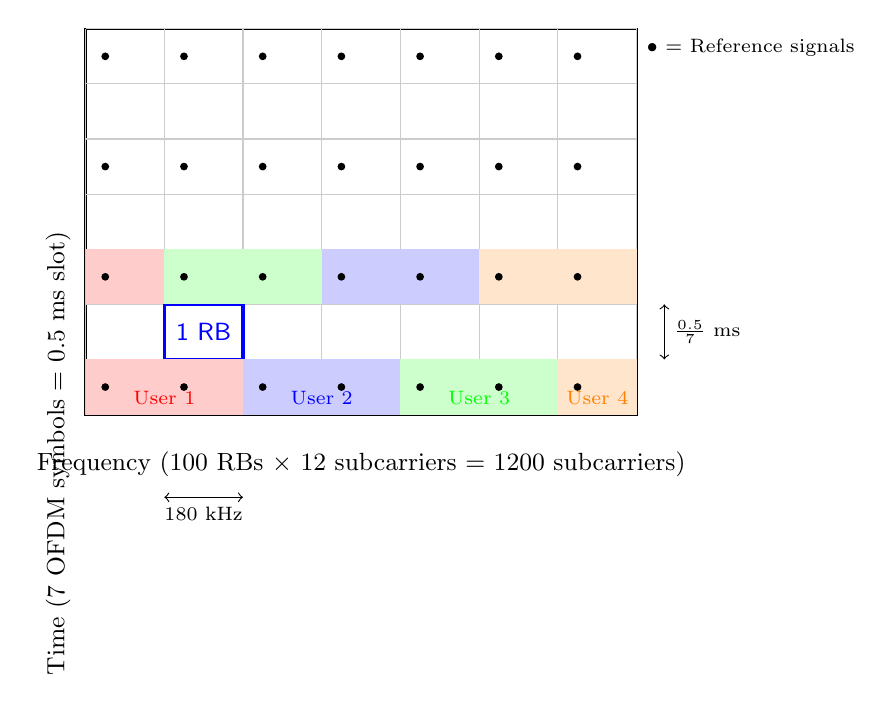
\begin{tikzpicture}[scale=0.7]
% LTE Resource Grid
\draw[thick] (0,0) rectangle (10,7);

% Draw grid
\foreach \x in {0,1.428,...,10} {
  \draw[thin,gray!40] (\x,0) -- (\x,7);
}
\foreach \y in {0,1,...,7} {
  \draw[thin,gray!40] (0,\y) -- (10,\y);
}

% Highlight one Resource Block
\draw[very thick,blue] (1.428,1) rectangle (2.856,2);
\node[blue,font=\sffamily\small] at (2.142,1.5) {1 RB};

% Color different RBs for different users
\fill[red!20] (0,0) rectangle (2.856,1);
\fill[blue!20] (2.856,0) rectangle (5.712,1);
\fill[green!20] (5.712,0) rectangle (8.568,1);
\fill[orange!20] (8.568,0) rectangle (10,1);

\fill[red!20] (0,2) rectangle (1.428,3);
\fill[green!20] (1.428,2) rectangle (4.284,3);
\fill[blue!20] (4.284,2) rectangle (7.14,3);
\fill[orange!20] (7.14,2) rectangle (10,3);

% Reference signals (pilots)
\foreach \x in {0.357,1.785,3.213,4.641,6.069,7.497,8.925} {
  \foreach \y in {0.5,2.5,4.5,6.5} {
    \fill[black] (\x,\y) circle (2pt);
  }
}

% Labels
\node[below,font=\small] at (5,-0.5) {Frequency (100 RBs $\times$ 12 subcarriers = 1200 subcarriers)};
\node[rotate=90,left,font=\small] at (-0.5,3.5) {Time (7 OFDM symbols = 0.5~ms slot)};

% User labels
\node[font=\scriptsize,red] at (1.428,0.3) {User 1};
\node[font=\scriptsize,blue] at (4.284,0.3) {User 2};
\node[font=\scriptsize,green] at (7.14,0.3) {User 3};
\node[font=\scriptsize,orange] at (9.284,0.3) {User 4};

% Dimensions
\draw[<->] (2.856,-1.5) -- (1.428,-1.5) node[midway,below,font=\scriptsize] {180~kHz};
\draw[<->] (10.5,1) -- (10.5,2) node[midway,right,font=\scriptsize] {$\frac{0.5}{7}$~ms};

% Legend
\node[below right,font=\scriptsize] at (10,7) {$\bullet$ = Reference signals};
\end{tikzpicture}
\end{center}

\begin{calloutbox}[colback=blue!5!white,colframe=blue!75!black]{Time-Frequency Resource Allocation}
The eNodeB scheduler assigns RBs dynamically every 1~ms (subframe):
\begin{itemize}
\item \textbf{User 1} (cell edge): Allocated 20 RBs with QPSK $\rightarrow$ 3~Mbps
\item \textbf{User 2} (mid-cell): Allocated 30 RBs with 16-QAM $\rightarrow$ 12~Mbps
\item \textbf{User 3} (near base): Allocated 25 RBs with 64-QAM $\rightarrow$ 15~Mbps
\item \textbf{User 4} (stationary): Allocated 25 RBs with 64-QAM $\rightarrow$ 15~Mbps
\end{itemize}

Total cell throughput: 45~Mbps with 4 active users, adapting MCS based on individual channel quality.
\end{calloutbox}

\subsubsection{Modulation \& Coding}\label{modulation-coding}

\textbf{MCS table} (QPSK to 64-QAM):

{\def\LTcaptype{} % do not increment counter
\begin{longtable}[]{@{}lllll@{}}
\toprule\noalign{}
MCS & Modulation & Code Rate & Spectral Eff. & Usage \\
\midrule\noalign{}
\endhead
\bottomrule\noalign{}
\endlastfoot
0 & QPSK & 0.08 & 0.15 & Cell edge \\
5 & QPSK & 0.37 & 0.74 & \\
10 & 16-QAM & 0.48 & 1.91 & Mid-cell \\
15 & 16-QAM & 0.74 & 2.96 & \\
20 & 64-QAM & 0.55 & 3.32 & Near base station \\
25 & 64-QAM & 0.85 & 5.12 & \\
28 & 64-QAM & 0.93 & 5.55 & Max throughput \\
\end{longtable}
}

\textbf{Adaptive MCS}: eNB (base station) selects based on CQI (Channel
Quality Indicator) reports

\begin{center}\rule{0.5\linewidth}{0.5pt}\end{center}

\subsection{Link Budget: Urban Macrocell}

\textbf{Scenario:} Downlink from macrocell tower to indoor smartphone at 1~km distance, 2~GHz band

\subsubsection*{Given Parameters}

\begin{tabular}{@{}ll@{}}
eNodeB TX power & $P_t = 46$~dBm (40~W total, 20~W per sector) \\
eNodeB antenna gain & $G_t = 17$~dBi (120° sector antenna) \\
Cable loss & $L_{\text{cable}} = 3$~dB \\
Distance & $d = 1$~km \\
Frequency & $f = 2.0$~GHz \\
Bandwidth & $B = 20$~MHz \\
UE antenna gain & $G_r = 0$~dBi (omnidirectional phone antenna) \\
UE noise figure & $NF = 9$~dB \\
Building penetration loss & $L_{\text{building}} = 15$~dB \\
Urban clutter loss & $L_{\text{urban}} = 20$~dB \\
\end{tabular}

\subsubsection*{Step 1: EIRP Calculation}

\begin{equation}
\text{EIRP} = P_t + G_t - L_{\text{cable}} = 46 + 17 - 3 = 60~\text{dBm}
\end{equation}

\subsubsection*{Step 2: Path Loss}

Free-space path loss:
\begin{equation}
\text{FSPL} = 20\log_{10}(1000) + 20\log_{10}(2000) + 32.45 = 60 + 66.0 + 32.45 = 92.0~\text{dB}
\end{equation}

Total path loss including propagation environment:
\begin{equation}
L_{\text{total}} = \text{FSPL} + L_{\text{urban}} + L_{\text{building}} = 92 + 20 + 15 = 127~\text{dB}
\end{equation}

\subsubsection*{Step 3: Received Signal Power}

\begin{equation}
P_r = \text{EIRP} + G_r - L_{\text{total}} = 60 + 0 - 127 = -67~\text{dBm}
\end{equation}

\subsubsection*{Step 4: Noise Power}

\begin{equation}
N = -174 + 10\log_{10}(20 \times 10^6) + 9 = -174 + 73.0 + 9 = -92~\text{dBm}
\end{equation}

\subsubsection*{Step 5: SNR and MCS Selection}

\begin{equation}
\text{SNR} = P_r - N = -67 - (-92) = 25~\text{dB}
\end{equation}

With 25~dB SNR, the scheduler selects:
\begin{itemize}
\item \textbf{MCS 23:} 64-QAM with code rate $r = 0.7$
\item \textbf{Spectral efficiency:} $\eta = 6 \times 0.7 = 4.2$~bits/s/Hz
\end{itemize}

\subsubsection*{Step 6: Data Rate Calculation}

For $2 \times 2$ MIMO with 100 RBs allocated:
\begin{equation}
R = N_{\text{RB}} \times N_{\text{sc}} \times N_{\text{sym}} \times M \times r \times N_{\text{layers}} / T_{\text{slot}}
\end{equation}
\begin{equation}
R = 100 \times 12 \times 7 \times 6 \times 0.7 \times 2 / 0.5~\text{ms} = 141,120 / 0.5 = 141.1~\text{Mbps}
\end{equation}

After accounting for reference signals, control overhead, and protocol layers:
\begin{equation}
R_{\text{MAC}} \approx 0.7 \times 141.1 \approx 100~\text{Mbps}
\end{equation}

\begin{calloutbox}{LTE Link Budget Summary}
\textbf{Result: 100~Mbps achievable at 1~km with 25~dB SNR}

This link operates in a \textbf{coverage-limited} regime:
\begin{itemize}
\item Cell-edge users (weak signal): Use QPSK, achieve $\sim$5~Mbps
\item Mid-cell users (moderate signal): Use 16-QAM, achieve $\sim$20--40~Mbps
\item Near-tower users (strong signal): Use 64-QAM, achieve 80--100~Mbps
\end{itemize}

\textbf{Handover margins:} LTE maintains soft handover with $\sim$3~dB hysteresis to prevent ping-ponging between cells at speeds up to 350~km/h.
\end{calloutbox}

\subsubsection{Synchronization \& Cell
Search}\label{synchronization-cell-search}

\textbf{Steps}:

\begin{enumerate}
\def\labelenumi{\arabic{enumi}.}
\tightlist
\item
  \textbf{PSS detection} (Primary Sync Signal):

  \begin{itemize}
  \tightlist
  \item
    3 Zadoff-Chu sequences (cell ID mod 3)
  \item
    Every 5 ms
  \item
    Coarse timing (\$\textbackslash pm\$5 ms ambiguity)
  \item
    Coarse CFO (from PSS phase)
  \end{itemize}
\item
  \textbf{SSS detection} (Secondary Sync Signal):

  \begin{itemize}
  \tightlist
  \item
    168 sequences (cell ID = 0-503)
  \item
    Frame timing (resolve 5 ms ambiguity)
  \item
    Cell ID fully determined
  \end{itemize}
\item
  \textbf{PBCH decode} (Physical Broadcast Channel):

  \begin{itemize}
  \tightlist
  \item
    Master Information Block (MIB)
  \item
    Bandwidth, PHICH config, frame number
  \item
    QPSK, rate 1/48 (very robust)
  \end{itemize}
\end{enumerate}

\textbf{Time}: \textasciitilde100 ms (cold start), \textasciitilde10 ms
(known frequency)

\begin{center}\rule{0.5\linewidth}{0.5pt}\end{center}

\subsubsection{Channel Estimation}\label{channel-estimation}

\textbf{Cell-Specific Reference Signals (CRS)}: - 4 pilots per RB per
OFDM symbol (port 0) - 8 pilots for 2\$\textbackslash times\$2 MIMO
(ports 0, 1)

\textbf{Estimation}: - LS per pilot: \(\hat{H}_p = R_p / S_p\) - Wiener
interpolation (frequency + time) - Averaging over multiple OFDM symbols
(4 ms)

\textbf{Tracking}: Phase/frequency drift (up to 300 km/h Doppler)

\begin{center}\rule{0.5\linewidth}{0.5pt}\end{center}

\subsubsection{Equalization (Downlink)}\label{equalization-downlink}

\textbf{Frequency domain} (per subcarrier):

\[
\hat{S}_k = \frac{H_k^*}{|H_k|^2 + \sigma^2} R_k \quad (\text{MMSE})
\]

\textbf{MIMO} (2\$\textbackslash times\$2): Per-subcarrier matrix
inversion

\textbf{Interference}: ICIC (Inter-Cell Interference Coordination)

\begin{center}\rule{0.5\linewidth}{0.5pt}\end{center}

\subsubsection{Performance}\label{performance-1}

\textbf{Throughput} (Cat 3, 2\$\textbackslash times\$2 MIMO, 20 MHz): -
\textbf{Peak}: 100 Mbps (downlink), 50 Mbps (uplink) - \textbf{Average}:
30-50 Mbps (loaded cell)

\textbf{Latency}: - Control plane: \textasciitilde50 ms (idle
\$\textbackslash rightarrow\$ active) - User plane: \textasciitilde10 ms
(round-trip)

\textbf{Range}: - \textbf{Macrocell}: 5-15 km (rural), 1-3 km (urban) -
\textbf{Small cell}: 100-500 m

\textbf{Handover}: \textasciitilde50 ms (seamless at \textless{} 300
km/h)

\begin{center}\rule{0.5\linewidth}{0.5pt}\end{center}

\subsection{3. DVB-S2X (Satellite TV, 4K
UHD)}\label{dvb-s2x-satellite-tv-4k-uhd}

\subsubsection{System Parameters}\label{system-parameters-2}

\textbf{Standard}: ETSI EN 302 307-2 (2014)

\textbf{Frequency}: Ku-band (10.7-12.75 GHz downlink)

\textbf{Bandwidth}: 36 MHz (transponder)

\textbf{Modulation}: QPSK, 8PSK, 16APSK, 32APSK (ACM, Adaptive Coding \&
Modulation)

\textbf{Coding}: LDPC + BCH (outer)

\textbf{Multiple access}: TDM (Time Division Multiplex, single carrier
per transponder)

\begin{center}\rule{0.5\linewidth}{0.5pt}\end{center}

\subsubsection{Frame Structure}\label{frame-structure-1}

\textbf{PLFRAME} (Physical Layer Frame): - PLHEADER (90 symbols): Frame
sync, MODCOD (modulation + code rate) - Pilots: 36 symbols every 1440
data symbols - Data: 16,200 or 64,800 bits (FECFRAME)

\textbf{Super-frame}: VCM (Variable Coding \& Modulation) allows
different MODCOD per frame

\begin{center}\rule{0.5\linewidth}{0.5pt}\end{center}

\subsubsection{Modulation \& Coding}\label{modulation-coding-1}

\textbf{MODCOD table} (examples):

{\def\LTcaptype{} % do not increment counter
\begin{longtable}[]{@{}lllll@{}}
\toprule\noalign{}
MODCOD & Modulation & Code Rate & Spectral Eff. & C/N Req. (dB) \\
\midrule\noalign{}
\endhead
\bottomrule\noalign{}
\endlastfoot
1 & QPSK & 1/4 & 0.49 & -2.3 \\
6 & QPSK & 3/4 & 1.49 & +4.0 \\
11 & 8PSK & 2/3 & 2.00 & +7.9 \\
17 & 8PSK & 9/10 & 2.69 & +12.7 \\
23 & 16APSK & 5/6 & 3.32 & +14.4 \\
28 & 32APSK & 9/10 & 4.48 & +18.4 \\
\end{longtable}
}

\textbf{ACM}: Switch MODCOD based on rain fade - Clear sky: 32APSK 9/10
(max throughput) - Light rain: 8PSK 3/4 - Heavy rain: QPSK 1/2

\begin{center}\rule{0.5\linewidth}{0.5pt}\end{center}

\subsubsection{Link Budget (GEO, Ku-Band, 4K
UHD)}\label{link-budget-geo-ku-band-4k-uhd}

\textbf{Satellite}: - TX power: +50 dBW (100 kW EIRP, 100 W transponder)
- Antenna gain: +35 dBi (spot beam) - EIRP: +85 dBW

\textbf{Path Loss} (GEO, 36,000 km, 12 GHz): - FSPL: 205.6 dB

\textbf{Ground Station}: - Dish size: 0.6 m (residential) - Antenna
gain: +37.4 dBi (60\% efficiency) - Pointing loss: -0.5 dB - RX gain:
+36.9 dBi - LNB noise temp: 50 K (NF \$\textbackslash approx\$ 0.7 dB) -
System temp: 150 K (sky + LNB) - G/T: +13.1 dB/K

\textbf{Received C/N} (Carrier-to-Noise): - C = 85 - 205.6 + 36.9 =
\textbf{-83.7 dBW} - N = -228.6 + 10log(36e6) + 10log(150) =
\textbf{-147.3 dBW} - \textbf{C/N = 63.6 dB} (clear sky, theoretical)

\textbf{With rain} (5 dB rain fade @ 12 GHz, 0.01\% time): - C/N = 63.6
- 5 = \textbf{58.6 dB} (still excellent!)

\textbf{MODCOD selection}: - Clear sky: 32APSK 9/10 (requires 18.4 dB
C/N) - Rain: 8PSK 2/3 (requires 7.9 dB C/N)

\textbf{Data rate}: - 32APSK 9/10: 36 MHz \$\textbackslash times\$ 4.48
= \textbf{161 Mbps} - Enough for 4K UHD (50 Mbps HEVC) + multiple HD
channels

\begin{center}\rule{0.5\linewidth}{0.5pt}\end{center}

\subsubsection{Synchronization}\label{synchronization-1}

\textbf{PLHEADER} (90 symbols): - Known pattern (SOF, Start of Frame) -
Correlate for frame sync - Acquire in \textasciitilde1 second (blind
search \$\textbackslash pm\$500 kHz CFO)

\textbf{Pilot symbols}: Every 16 data symbols (distributed) -
Phase/frequency tracking - Common phase error (CPE) correction

\begin{center}\rule{0.5\linewidth}{0.5pt}\end{center}

\subsubsection{Equalization}\label{equalization-1}

\textbf{Single carrier} (not OFDM): - Phase noise dominant (satellite
oscillator, ground LNB) - Decision-directed phase tracking - Pilot-aided
(every 16 symbols)

\textbf{Channel}: Mostly flat (GEO, line-of-sight, no multipath)

\begin{center}\rule{0.5\linewidth}{0.5pt}\end{center}

\subsubsection{Performance}\label{performance-2}

\textbf{Availability}: 99.7\% (0.3\% outage in heavy rain)

\textbf{Latency}: \textasciitilde600 ms (round-trip to GEO and back)

\textbf{Throughput}: 80-160 Mbps (depends on MODCOD, ACM)

\textbf{Spectral efficiency}: 1.5-4.5 bits/sec/Hz

\begin{center}\rule{0.5\linewidth}{0.5pt}\end{center}

\subsection{4. GPS L1 C/A (Civilian
Navigation)}\label{gps-l1-ca-civilian-navigation}

\subsubsection{System Parameters}\label{system-parameters-3}

\textbf{Standard}: IS-GPS-200 (US DoD)

\textbf{Frequency}: L1 = 1575.42 MHz

\textbf{Bandwidth}: 2.046 MHz (C/A code)

\textbf{Modulation}: BPSK (data) on DSSS (Direct Sequence Spread
Spectrum)

\textbf{Spreading}: 1.023 Mcps (C/A Gold code, 1023 chips)

\textbf{Data rate}: 50 bps (navigation message)

\textbf{Code rate}: None (no FEC on nav message, 1/2 rate implied by
chip parity in modern receivers)

\begin{center}\rule{0.5\linewidth}{0.5pt}\end{center}

\subsubsection{Signal Structure}\label{signal-structure}

\textbf{C/A code}: 1023-chip Gold code (repeats every 1 ms) - Unique
code per satellite (32 satellites, \textasciitilde30 visible codes) -
Chip rate: 1.023 Mcps - Chip duration: \textasciitilde977 ns

\textbf{Navigation data}: 50 bps - 20 ms per bit (20 C/A code
repetitions) - Preamble, ephemeris, almanac

\textbf{Spreading}:

\[
s(t) = d(t) \cdot c(t) \cdot \cos(2\pi f_L1 t)
\]

Where: - \(d(t)\) = Navigation data (\$\textbackslash pm\$1) - \(c(t)\)
= C/A code (\$\textbackslash pm\$1, 1.023 Mcps)

\begin{center}\rule{0.5\linewidth}{0.5pt}\end{center}

\subsubsection{Link Budget}\label{link-budget}

\textbf{Satellite} (MEO, 20,200 km): - TX power: +27 dBW (500 W
spacecraft, 50 W to L1) - Antenna gain: +13 dBi (earth-facing) - EIRP:
+40 dBW

\textbf{Path Loss} (1.575 GHz, 20,200 km): - FSPL: 184 dB

\textbf{Receiver} (handheld): - Antenna gain: +3 dBi (patch antenna) -
Cable loss: -2 dB - RX gain: +1 dBi - Noise figure: 3 dB - Noise floor:
-174 + 63 + 3 = -108 dBm (2 MHz)

\textbf{Received signal}: - P\_r = 40 - 184 + 1 = \textbf{-143 dBm}

\textbf{SNR} (before despreading): -143 - (-108) = \textbf{-35 dB}

\textbf{Processing gain} (despreading): - G\_p = 10log(1.023e6 / 50) =
\textbf{43 dB}

\textbf{SNR after despreading}: -35 + 43 = \textbf{+8 dB}

\textbf{Enough for}: BER
\textasciitilde10\textbackslash textsuperscript\{-\}\textbackslash textsuperscript\{5\}
(BPSK @ 8 dB Eb/N0)

\begin{center}\rule{0.5\linewidth}{0.5pt}\end{center}

\subsubsection{Acquisition \& Tracking}\label{acquisition-tracking}

\textbf{Acquisition} (cold start):

\begin{enumerate}
\def\labelenumi{\arabic{enumi}.}
\tightlist
\item
  \textbf{Search space}:

  \begin{itemize}
  \tightlist
  \item
    Doppler: \$\textbackslash pm\$5 kHz (satellite motion)
  \item
    Code phase: 0-1022 chips (1 ms uncertainty)
  \item
    Total: 5000 \$\textbackslash times\$ 1023 = \textbf{5.1 million
    hypotheses}
  \end{itemize}
\item
  \textbf{FFT-based search}:

  \begin{itemize}
  \tightlist
  \item
    Correlate 1 ms of signal with local code (FFT)
  \item
    Sweep Doppler (500 Hz steps)
  \item
    \textbf{Time}: \textasciitilde1 second per satellite (parallel
    correlators)
  \end{itemize}
\item
  \textbf{Threshold}: Peak exceeds noise floor by 10 dB
  \$\textbackslash rightarrow\$ Satellite acquired
\end{enumerate}

\textbf{Tracking}:

\begin{itemize}
\tightlist
\item
  \textbf{DLL} (Delay-Locked Loop): Code phase (\$\textbackslash pm\$0.5
  chip)
\item
  \textbf{PLL} (Phase-Locked Loop): Carrier phase (sub-wavelength,
  \textasciitilde19 cm)
\item
  \textbf{FLL} (Frequency-Locked Loop): Doppler
  (\$\textbackslash pm\$0.1 Hz)
\end{itemize}

\textbf{Update}: 1 kHz (1 ms integration)

\begin{center}\rule{0.5\linewidth}{0.5pt}\end{center}

\subsubsection{Navigation Solution}\label{navigation-solution}

\textbf{Minimum 4 satellites}: Solve for (x, y, z, clock bias)

\textbf{Pseudorange} (from code phase):

\[
\rho_i = c \cdot \Delta t_i = \sqrt{(x - x_i)^2 + (y - y_i)^2 + (z - z_i)^2} + c \cdot b
\]

Where: - \(\rho_i\) = Measured pseudorange to satellite \(i\) -
\((x, y, z)\) = User position - \((x_i, y_i, z_i)\) = Satellite position
(from ephemeris) - \(b\) = User clock bias

\textbf{Solve} (least squares, iterative):

\[
\mathbf{p} = (\mathbf{H}^T \mathbf{H})^{-1} \mathbf{H}^T \Delta\boldsymbol{\rho}
\]

\textbf{Accuracy}: - \textbf{Horizontal}: 5-10 m (standalone,
unencrypted C/A) - \textbf{With DGPS}: 1-3 m (differential corrections)
- \textbf{With RTK}: 1-10 cm (carrier phase, short baseline)

\begin{center}\rule{0.5\linewidth}{0.5pt}\end{center}

\subsubsection{Performance}\label{performance-3}

\textbf{Time to first fix} (TTFF): - \textbf{Cold start}: 30-60 seconds
(no almanac) - \textbf{Warm start}: 10-30 seconds (old almanac) -
\textbf{Hot start}: 1-10 seconds (recent ephemeris)

\textbf{Update rate}: 1 Hz (can be 10 Hz with modern receivers)

\subsubsection{External Resources}\label{external-resources}

\textbf{GPS Technical Documentation}: -
\href{https://www.gps.gov/technical/icwg/IS-GPS-200M.pdf}{IS-GPS-200
Interface Specification} - Official GPS signal specification -
\href{https://www.gps.gov/}{GPS.gov} - U.S. government GPS information
portal -
\href{https://gssc.esa.int/navipedia/index.php?title=GPS}{Navipedia GPS
Section} - Comprehensive GPS technical resource

\textbf{Related GNSS Systems}: -
\href{https://www.gsc-europa.eu/sites/default/files/sites/all/files/Galileo_OS_SIS_ICD_v2.0.pdf}{Galileo
OS SIS ICD} - European GNSS signal plan -
\href{https://gssc.esa.int/navipedia/index.php?title=GALILEO_Signal_Plan}{Navipedia
Signal Plan Comparison} - Multi-GNSS signal analysis

\textbf{Sensitivity}: -130 dBm (open sky), -145 dBm (aided, indoor
marginal)

\begin{center}\rule{0.5\linewidth}{0.5pt}\end{center}

\subsection{5. Bluetooth 5.0 (LE Audio)}\label{bluetooth-5.0-le-audio}

\subsubsection{System Parameters}\label{system-parameters-4}

\textbf{Standard}: Bluetooth 5.0 (2016), LE Audio (2020)

\textbf{Frequency}: 2.4 GHz ISM band (2400-2483.5 MHz)

\textbf{Bandwidth}: 2 MHz per channel (40 channels, 2 MHz spacing)

\textbf{Modulation}: GFSK (Gaussian Frequency Shift Keying, BT=0.5)

\textbf{Data rate}: 1 Mbps (LE 1M), 2 Mbps (LE 2M), 125/500 kbps (LE
Coded)

\textbf{Coding}: None (1M, 2M), FEC S=2 or S=8 (LE Coded)

\textbf{Range}: 10-100 m (LE), 200-400 m (LE Long Range)

\begin{center}\rule{0.5\linewidth}{0.5pt}\end{center}

\subsubsection{Modulation}\label{modulation}

\textbf{GFSK} (Gaussian FSK): - \textbf{Deviation}:
\$\textbackslash pm\$250 kHz (1M), \$\textbackslash pm\$500 kHz (2M) -
\textbf{Modulation index}: h = 0.5 (1M), h = 1.0 (2M) - \textbf{Gaussian
BT}: 0.5 (pre-filter to reduce bandwidth)

\textbf{Bit 0}: -250 kHz (1M)

\textbf{Bit 1}: +250 kHz (1M)

\textbf{Receiver}: FM discriminator (non-coherent) or coherent (better
sensitivity)

\begin{center}\rule{0.5\linewidth}{0.5pt}\end{center}

\subsubsection{Frame Structure}\label{frame-structure-2}

\textbf{Advertising packet} (connection initiation): - Preamble: 8 bits
(01010101 for 1M) - Access address: 32 bits (0x8E89BED6 for advertising)
- PDU: 2-39 bytes (header + payload) - CRC: 24 bits

\textbf{Data packet} (connection): - Preamble: 8 bits - Access address:
32 bits (unique per connection) - PDU: 2-255 bytes - CRC: 24 bits

\textbf{FEC} (LE Coded): - S=2: Rate 1/2, block code - S=8: Rate 1/8,
repetition code

\begin{center}\rule{0.5\linewidth}{0.5pt}\end{center}

\subsubsection{Link Budget (LE 1M, 10 m)}\label{link-budget-le-1m-10-m}

\textbf{Transmitter} (phone): - TX power: 0 dBm (1 mW, class 2) -
Antenna gain: 0 dBi (PCB antenna) - EIRP: 0 dBm

\textbf{Path Loss} (10 m indoor, 2.4 GHz): - Free space: 40 dB - Indoor
clutter: 10 dB - \textbf{Total}: 50 dB

\textbf{Receiver} (headphones): - RX antenna gain: 0 dBi - Noise figure:
12 dB (low-power design) - Noise floor: -174 + 63 + 12 = -99 dBm (2 MHz)

\textbf{Received signal}: - P\_r = 0 - 50 + 0 = \textbf{-50 dBm}

\textbf{SNR}: -50 - (-99) = \textbf{49 dB} (excellent!)

\textbf{Sensitivity} (spec): -70 dBm (1M), -80 dBm (LE Coded S=8)

\textbf{Margin}: 49 - 19 = \textbf{30 dB} (19 dB SNR needed for
10\textbackslash textsuperscript\{-\}\textbackslash textsuperscript\{3\}
BER)

\begin{center}\rule{0.5\linewidth}{0.5pt}\end{center}

\subsubsection{Synchronization}\label{synchronization-2}

\textbf{Preamble}: 8-bit alternating pattern (01010101 or 10101010) -
Frequency offset estimation - Timing sync (bit transitions)

\textbf{Access address}: 32-bit correlation - Frame detection - Fine
timing

\textbf{CFO tolerance}: \$\textbackslash pm\$50 ppm - @ 2.4 GHz:
\$\textbackslash pm\$120 kHz - Channel BW: 2 MHz - Correctable with
preamble estimation

\begin{center}\rule{0.5\linewidth}{0.5pt}\end{center}

\subsubsection{Adaptive Frequency Hopping
(AFH)}\label{adaptive-frequency-hopping-afh}

\textbf{Avoid interference} from WiFi:

\textbf{Channel hopping}: Pseudo-random sequence, 37 data channels - Hop
every 1.25 ms (connection event) - Bad channels blacklisted (CCA, Clear
Channel Assessment)

\textbf{Example}: WiFi on ch 6 (2437 MHz, 20 MHz BW) - BT avoids ch
15-24 (2428-2456 MHz) - Uses remaining 27 channels

\begin{center}\rule{0.5\linewidth}{0.5pt}\end{center}

\subsubsection{Performance}\label{performance-4}

\textbf{Throughput}: - \textbf{LE 1M}: \textasciitilde700 kbps
(application layer, overhead \textasciitilde30\%) - \textbf{LE 2M}:
\textasciitilde1.4 Mbps - \textbf{LE Coded S=2}: \textasciitilde350 kbps
- \textbf{LE Coded S=8}: \textasciitilde100 kbps

\textbf{Latency}: 7.5-40 ms (connection interval)

\textbf{Range}: - \textbf{LE 1M}: 10-30 m (typical), 100 m (outdoor,
LoS) - \textbf{LE Long Range (S=8)}: 200-400 m (outdoor)

\textbf{Power}: 10-50 mW (active), \textless{} 1 \$\textbackslash mu\$W
(deep sleep)

\begin{center}\rule{0.5\linewidth}{0.5pt}\end{center}

\subsection{6. LoRaWAN (IoT Long Range)}\label{lorawan-iot-long-range}

\subsubsection{System Parameters}\label{system-parameters-5}

\textbf{Standard}: LoRa Alliance (2015)

\textbf{Frequency}: ISM bands (433, 868, 915 MHz)

\textbf{Bandwidth}: 125, 250, 500 kHz

\textbf{Modulation}: LoRa (Chirp Spread Spectrum, proprietary Semtech)

\textbf{Data rate}: 0.3-50 kbps (adaptive)

\textbf{Coding}: FEC rate 4/5, 4/6, 4/7, 4/8 (Hamming-based)

\textbf{Range}: 2-15 km (urban), 30-50 km (rural, LoS)

\begin{center}\rule{0.5\linewidth}{0.5pt}\end{center}

\subsubsection{LoRa Modulation}\label{lora-modulation}

\textbf{CSS} (Chirp Spread Spectrum): - Frequency sweeps linearly across
bandwidth - \textbf{Symbol duration}: \(T_s = 2^{SF} / BW\) -
\textbf{SF} (Spreading Factor): 7-12 (trade data rate vs range)

\textbf{Example} (SF=7, BW=125 kHz): - \(T_s = 2^7 / 125000 = 1.024\) ms
- Data rate: 5.47 kbps (rate 4/5 coding)

\textbf{Example} (SF=12, BW=125 kHz): -
\(T_s = 2^{12} / 125000 = 32.768\) ms - Data rate: 0.25 kbps

\textbf{Energy per bit}: Higher SF \$\textbackslash rightarrow\$ More
energy per bit \$\textbackslash rightarrow\$ Longer range

\begin{center}\rule{0.5\linewidth}{0.5pt}\end{center}

\subsubsection{Link Budget (SF12, 868 MHz, 15
km)}\label{link-budget-sf12-868-mhz-15-km}

\textbf{End Device} (sensor): - TX power: +14 dBm (25 mW, EU limit) -
Antenna gain: +2 dBi (whip antenna) - EIRP: +16 dBm

\textbf{Path Loss} (15 km rural, 868 MHz): - Free space: 111 dB -
Terrain: 20 dB (rolling hills) - \textbf{Total}: 131 dB

\textbf{Gateway} (base station): - RX antenna gain: +8 dBi (omni or
sector) - Cable loss: -1 dB - RX gain: +7 dBi - Noise figure: 3 dB
(SX1301) - Noise floor: -174 + 51 + 3 = -120 dBm (125 kHz)

\textbf{Received signal}: - P\_r = 16 - 131 + 7 = \textbf{-108 dBm}

\textbf{SNR}: -108 - (-120) = \textbf{12 dB}

\textbf{Required SNR} (SF12): -20 dB (yes, negative! CSS allows
below-noise detection)

\textbf{Margin}: 12 - (-20) = \textbf{32 dB}

\textbf{Range}: 15 km achievable

\begin{center}\rule{0.5\linewidth}{0.5pt}\end{center}

\subsubsection{Adaptive Data Rate (ADR)}\label{adaptive-data-rate-adr}

\textbf{Network server adjusts} SF and TX power per device:

{\def\LTcaptype{} % do not increment counter
\begin{longtable}[]{@{}llll@{}}
\toprule\noalign{}
SF & Data Rate & Range & Energy \\
\midrule\noalign{}
\endhead
\bottomrule\noalign{}
\endlastfoot
\textbf{7} & 5.5 kbps & 2 km & Low \\
\textbf{9} & 1.8 kbps & 5 km & Moderate \\
\textbf{12} & 0.25 kbps & 15 km & High \\
\end{longtable}
}

\textbf{Goal}: Minimize airtime and energy (battery life)

\textbf{Example}: Device near gateway - Start SF12 (robust) - Network
commands SF7 (after several successful packets) - Airtime: 32.7 ms
\$\textbackslash rightarrow\$ 1.0 ms (32\$\textbackslash times\$ faster)
- Battery life: 5\$\textbackslash times\$ improvement

\begin{center}\rule{0.5\linewidth}{0.5pt}\end{center}

\subsubsection{LoRaWAN Protocol}\label{lorawan-protocol}

\textbf{Class A} (battery): - Uplink \$\textbackslash rightarrow\$ 2 RX
windows (1s, 2s after TX) - Downlink only in RX windows - Power:
\textasciitilde100 mW-years (1 packet/hour)

\textbf{Class B} (synchronized): - Periodic RX slots (128 ms beacon from
gateway) - Latency: \textless{} 128 seconds

\textbf{Class C} (mains powered): - RX always on (except during TX) -
Latency: \textasciitilde1 second

\begin{center}\rule{0.5\linewidth}{0.5pt}\end{center}

\subsubsection{Performance}\label{performance-5}

\textbf{Range}: - \textbf{Urban}: 2-5 km (SF7), 5-15 km (SF12) -
\textbf{Rural}: 10-30 km (line-of-sight, SF12) - \textbf{Record}: 702 km
(high altitude balloon, extreme conditions)

\textbf{Capacity}: \textasciitilde1000 devices per gateway (duty cycle
limited)

\textbf{Battery life}: 5-15 years (1 packet/hour,
3\$\textbackslash times\$AA batteries)

\textbf{Latency}: 1-10 seconds (Class A, includes ADR negotiation)

\begin{center}\rule{0.5\linewidth}{0.5pt}\end{center}

\subsection{Comparison Summary}\label{comparison-summary}

{\def\LTcaptype{} % do not increment counter
\begin{longtable}[]{@{}
  >{\raggedright\arraybackslash}p{(\linewidth - 14\tabcolsep) * \real{0.1096}}
  >{\raggedright\arraybackslash}p{(\linewidth - 14\tabcolsep) * \real{0.1507}}
  >{\raggedright\arraybackslash}p{(\linewidth - 14\tabcolsep) * \real{0.1507}}
  >{\raggedright\arraybackslash}p{(\linewidth - 14\tabcolsep) * \real{0.0959}}
  >{\raggedright\arraybackslash}p{(\linewidth - 14\tabcolsep) * \real{0.1644}}
  >{\raggedright\arraybackslash}p{(\linewidth - 14\tabcolsep) * \real{0.1096}}
  >{\raggedright\arraybackslash}p{(\linewidth - 14\tabcolsep) * \real{0.1233}}
  >{\raggedright\arraybackslash}p{(\linewidth - 14\tabcolsep) * \real{0.0959}}@{}}
\toprule\noalign{}
\begin{minipage}[b]{\linewidth}\raggedright
System
\end{minipage} & \begin{minipage}[b]{\linewidth}\raggedright
Frequency
\end{minipage} & \begin{minipage}[b]{\linewidth}\raggedright
Data Rate
\end{minipage} & \begin{minipage}[b]{\linewidth}\raggedright
Range
\end{minipage} & \begin{minipage}[b]{\linewidth}\raggedright
Modulation
\end{minipage} & \begin{minipage}[b]{\linewidth}\raggedright
Coding
\end{minipage} & \begin{minipage}[b]{\linewidth}\raggedright
Latency
\end{minipage} & \begin{minipage}[b]{\linewidth}\raggedright
Power
\end{minipage} \\
\midrule\noalign{}
\endhead
\bottomrule\noalign{}
\endlastfoot
\textbf{WiFi 802.11n} & 2.4/5 GHz & 65-600 Mbps & 10-100 m & 64-QAM OFDM
& Conv K=7 & 1-5 ms & 100 mW \\
\textbf{LTE} & 700-2600 MHz & 10-100 Mbps & 1-15 km & 64-QAM OFDMA &
Turbo K=4 & 10 ms & 200 mW \\
\textbf{DVB-S2X} & 12 GHz & 50-160 Mbps & 36,000 km & 32APSK & LDPC+BCH
& 600 ms & 100 W (sat) \\
\textbf{GPS L1} & 1.575 GHz & 50 bps & Global & BPSK DSSS & None & N/A &
50 W (sat) \\
\textbf{Bluetooth 5} & 2.4 GHz & 0.1-2 Mbps & 10-400 m & GFSK &
FEC/Repeat & 7-40 ms & 10 mW \\
\textbf{LoRaWAN} & 868/915 MHz & 0.3-50 kbps & 2-50 km & LoRa CSS &
Hamming & 1-10 s & 25 mW \\
\end{longtable}
}

\begin{center}\rule{0.5\linewidth}{0.5pt}\end{center}

\subsection{Key Takeaways by System}\label{key-takeaways-by-system}

\textbf{WiFi}: High throughput, OFDM handles multipath, MIMO for
capacity, short range

\textbf{LTE}: Cellular coverage, adaptive MCS, OFDMA multi-user,
handover at 300 km/h

\textbf{DVB-S2X}: Satellite broadcast, ACM for rain fade, long latency
(GEO), high EIRP

\textbf{GPS}: Below noise floor (-143 dBm), spread spectrum (43 dB
gain), 5-10 m accuracy

\textbf{Bluetooth}: Low power, AFH avoids WiFi, LE Coded for range, 7.5
ms latency

\textbf{LoRaWAN}: Ultra-long range (15+ km), sub-noise detection (CSS),
years battery life

\begin{center}\rule{0.5\linewidth}{0.5pt}\end{center}

\subsection{Related Topics}\label{related-topics}

\begin{itemize}
\tightlist
\item
  \textbf{{[}{[}Signal-Chain-(End-to-End-Processing){]}{]}}: System
  block diagrams
\item
  \textbf{{[}{[}Complete-Link-Budget-Analysis{]}{]}}: Detailed link
  calculations
\item
  \textbf{{[}{[}OFDM-\&-Multicarrier-Modulation{]}{]}}: WiFi/LTE PHY
  layer
\item
  \textbf{{[}{[}Spread-Spectrum-(DSSS-FHSS){]}{]}}: GPS, Bluetooth AFH
\item
  \textbf{{[}{[}Adaptive-Modulation-\&-Coding-(AMC){]}{]}}: LTE,
  DVB-S2X, LoRaWAN ADR
\end{itemize}

\begin{center}\rule{0.5\linewidth}{0.5pt}\end{center}

\subsection{External Resources \&
Standards}\label{external-resources-standards}

\subsubsection{WiFi (802.11)}\label{wifi-802.11}

\begin{itemize}
\tightlist
\item
  \href{https://standards.ieee.org/standard/802_11-2020.html}{IEEE
  802.11 Standards} - Official WiFi specifications
\item
  \href{https://www.wi-fi.org/}{WiFi Alliance} - Certification and
  technical information
\end{itemize}

\subsubsection{LTE/5G}\label{lte5g}

\begin{itemize}
\tightlist
\item
  \href{https://www.3gpp.org/ftp/Specs/archive/}{3GPP Specifications} -
  Complete LTE/5G standards
\item
  \href{https://www.3gpp.org/ftp/Specs/archive/36_series/36.211/}{3GPP
  TS 36.211} - LTE Physical channels and modulation
\item
  \href{https://www.3gpp.org/ftp/Specs/archive/36_series/36.212/}{3GPP
  TS 36.212} - LTE Channel coding
\end{itemize}

\subsubsection{DVB Satellite}\label{dvb-satellite}

\begin{itemize}
\tightlist
\item
  \href{https://www.etsi.org/deliver/etsi_en/302300_302399/30230701/}{ETSI
  EN 302 307-1} - DVB-S2 Standard
\item
  \href{https://www.dvb.org/}{DVB Project} - Digital Video Broadcasting
  organization
\end{itemize}

\subsubsection{Signal Identification}\label{signal-identification}

\begin{itemize}
\tightlist
\item
  \href{https://www.sigidwiki.com/wiki/Signal_Identification_Guide}{sigidwiki}
  - Comprehensive RF signal database
\item
  \href{https://www.radioreference.com/}{RadioReference} - Frequency
  allocations and trunked systems
\end{itemize}

\subsubsection{Full Bibliography}\label{full-bibliography}

\begin{itemize}
\tightlist
\item
  See {[}{[}Bibliography{]}{]} for complete list of 60+ references,
  textbooks, and resources
\end{itemize}

\begin{center}\rule{0.5\linewidth}{0.5pt}\end{center}

\textbf{Key takeaway}: \textbf{Real systems integrate all concepts:
modulation (BPSK to 256-QAM), coding (convolutional to LDPC), multiple
access (CSMA, OFDMA, TDMA), sync (preambles, pilots), equalization
(MMSE, DFE), and link budgets.} WiFi achieves 600 Mbps via MIMO + 64-QAM
OFDM over 100 m. LTE provides 100 Mbps cellular over 15 km with ACM.
DVB-S2X delivers 160 Mbps from GEO (36,000 km) using 32APSK. GPS
operates at -143 dBm (below noise!) via 43 dB spreading gain. Bluetooth
5 extends to 400 m with FEC (LE Coded). LoRaWAN reaches 50 km rural with
CSS sub-noise detection. Each system optimizes for different
constraints: throughput vs range vs power vs latency. Understanding
these trade-offs is key to system design!

\begin{center}\rule{0.5\linewidth}{0.5pt}\end{center}

\emph{This wiki is part of the {[}{[}Home\textbar Chimera Project{]}{]}
documentation.}
